\clearpage
\section{Casi d'uso}
\label{sec:user_case}
\subsection{Attori dei casi d'uso}
\label{sec:attori_uc}
\subsubsection{Attori primari}
%immagine gerarchio utilizzo + didascalia
\begin{itemize}
	\item  Utente generico: utente che, indipendentemente dal fatto che abbia effettuato il login o meno, accede all'applicazione;
	\item  Utente non autenticato: utente che non ha effettuato il login;
	\item  Utente autenticato: utente che ha completato la procedura di autenticazione.
\end{itemize}

%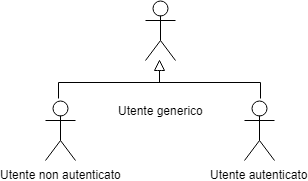
\includegraphics[width=1\textwidth]{../includes/pics/primari.png}
\begin{figure}[H]
	\centering
	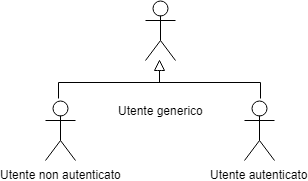
\includegraphics[width=10cm,keepaspectratio]{../includes/pics/primari.png}
	\caption{\label{fig:mission}Utenti del sistema}
\end{figure}

\begin{figure}[H]
	\centering
	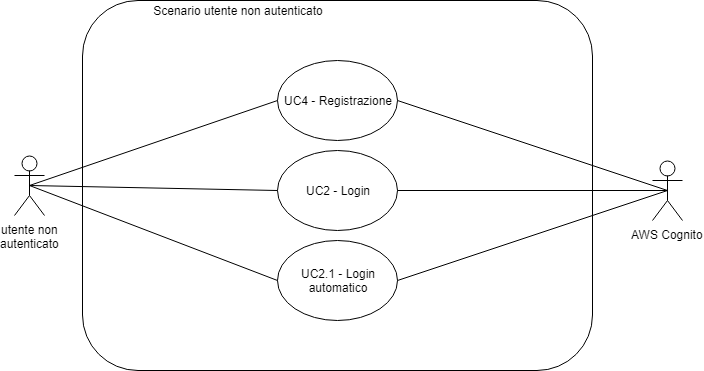
\includegraphics[width=15cm,keepaspectratio]{../includes/pics/scenario_non_autenticato.png}
	\caption{\label{fig:mission}Scenario per utente non autenticato}
\end{figure}

\begin{figure}[H]
	\centering
	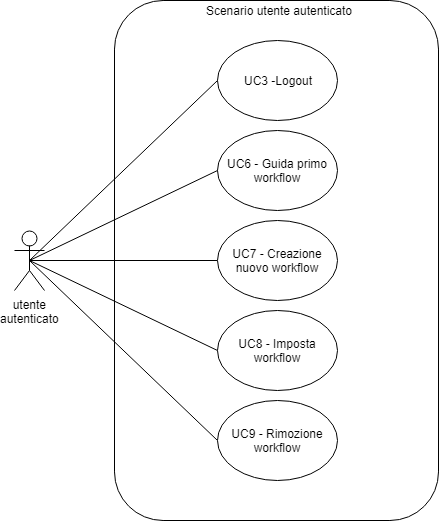
\includegraphics[width=15cm,keepaspectratio]{../includes/pics/scenario_autenticato.png}
	\caption{\label{fig:mission}Scenario per utente autenticato}
\end{figure}


\subsection{Elenco dei casi d'uso}
\label{sec:elenco_uc}
%immagine attori che accedono a casi d'uso+didascalia


\subsubsection{UC1 - Presentazione funzionalità}
\begin{itemize}
	\item  Attori primari: utente generico;
	\item  Scopo e descrizione: viene presentato all'utente una breve guida illustrata che permette di capire cosa è possibile fare con l'applicazione;
	\item  Scenario principale: l'utente visualizza la presentazione;
	\item  Pre-condizione: il sistema è funzionante e raggiungibile;
	\item  Post-condizione: l'utente è stato informato di alcune abilità del sistema.
\end{itemize}

%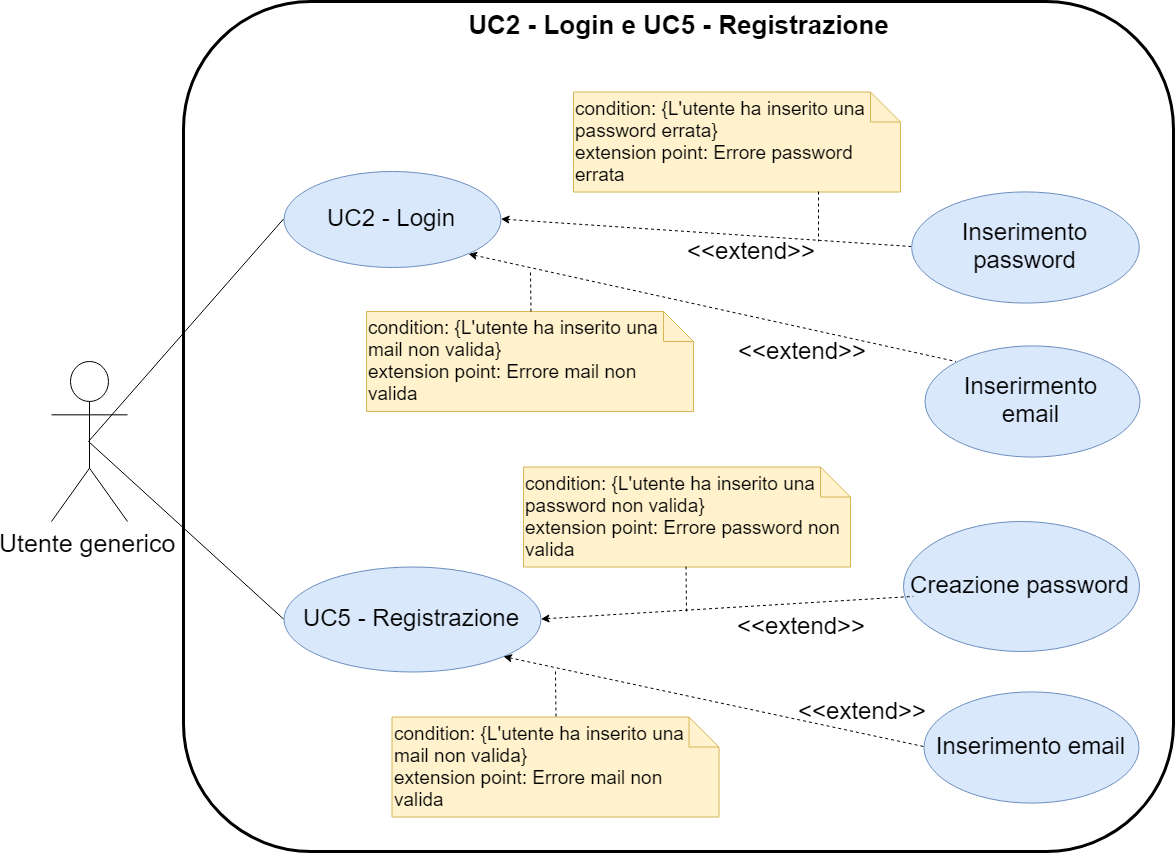
\includegraphics[width=1\textwidth]{../includes/pics/login_e_registrazione.png}
%\begin{figure}[H]
%	\centering
%	\includegraphics[width=15cm,keepaspectratio]%{../includes/pics/login_postRR.png}
%	\caption{\label{fig:mission}UC2 Login}
%\end{figure}

\subsubsection{UC2 - Login}
\begin{itemize}
	\item  Attori primari: utente non autenticato;
	\item  Attore secondario : AWS Cognito;
	\item  Scopo e descrizione: l' utente richiede il login al sistema attraverso AWS Cognito;
	\item  Scenario principale: l’utente non ancora riconosciuto dal sistema effettua il login;
		    
	\item  Pre-condizione: l'utente non è autenticato;
	\item  Post-condizione: l'utente è autenticato, viene riconosciuto dal sistema e accede alla sua bacheca.
\end{itemize}

\subsubsection{UC2.1 - Login automatico}
\begin{itemize}
	\item  Attori primari: utente non autenticato;
    \item  Attore secondario : AWS Cognito;
	\item  Scopo e descrizione: l'utente attende che di essere autenticato dal sistema attraverso AWS   Cognito;
	\item  Scenario principale: l'utente viene riconosciuto dal sistema senza che gli vengano richiesti i dati di accesso;
	\item  Pre-condizione: l'utente non è autenticato e ha effettuato il login in precedenza;
	\item  Post-condizione: l'utente è autenticato, viene riconosciuto dal sistema e accede alla sua bacheca.
\end{itemize}
\subsubsection{UC3 - Logout}
\begin{itemize}
	\item  Attori primari: utente autenticato;
    \item  Attore secondario : AWS Cognito;	
    \item  Scopo e descrizione: l'utente, tramite la pressione dell' opportuno bottone, termina la propria sessione con l'applicazione;
	\item  Scenario principale: l'utente effettua la procedura di de-autenticazione;
	\item  Pre-condizione: l'utente è autenticato e riconosciuto dal sistema;
	\item  Post-condizione: l'utente non è più autenticato e viene riportato al login di AWS Cognito.
\end{itemize}

%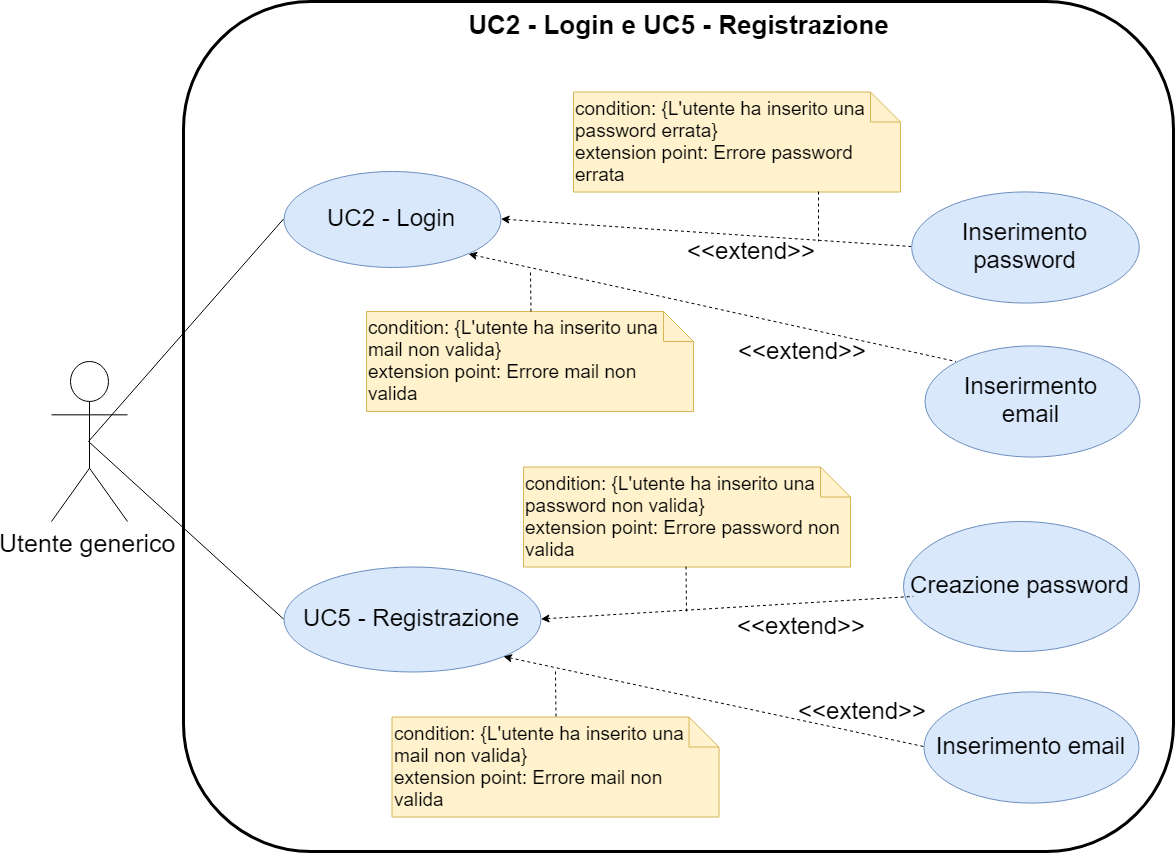
\includegraphics[width=1\textwidth]{../includes/pics/login_e_registrazione.png}
%\begin{figure}[H]
%	\centering
%	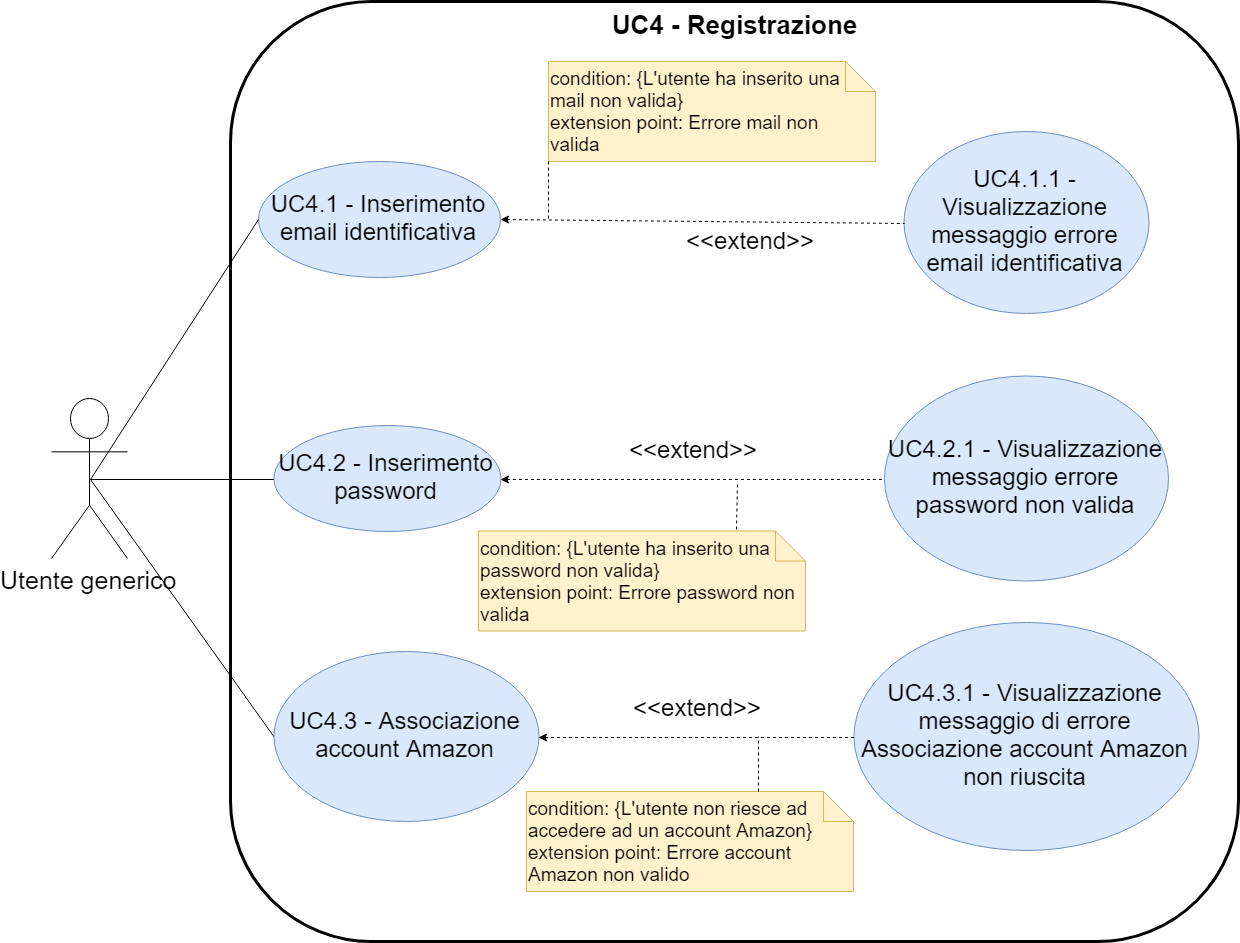
\includegraphics[width=15cm,keepaspectratio]{../includes/pics/registrazione_postRR.png}
%	\caption{\label{fig:mission}UC4 Registrazione}
%\end{figure}

\subsubsection{UC4 - Registrazione}
\begin{itemize}
	\item  Attori primari: utente non autenticato;
	\item  Attore secondario : AWS Cognito;
	\item  Scopo e descrizione: all'utente non autenticato viene presentato un form generato da AWS Cognito per effettuare la registrazione;
	\item  Scenario principale: l'utente inserisce i propri dati personali e segue i passaggi necessari per la registrazione;
	\item  Estensioni:
		   \begin{itemize}
		   	    \item se l'utente non ha una connessione stabile riceve un messaggio di errore [UC5];
		   \end{itemize}		    
	\item  Pre-condizione: l'utente non è autenticato ne registrato;
	\item  Post-condizione: l'utente è registrato e autenticato nel sistema, viene visualizzata la guida per il primo workflow [UC6].
\end{itemize}

\subsubsection{UC5 - Visualizzazione messaggio errore connessione}
\begin{itemize}
	\item  Attori primari: utente non autenticato;
	\item  Scopo e descrizione: l'utente viene avvisato che non è possibile accedere al sistema a causa di un errore di connessione;
	\item  Scenario principale: l'utente visualizza l'errore relativo alla mancanza di una connessione stabile;
	\item  Pre-condizione: l'utente vuole accedere al sistema senza avere una connessione internet disponibile;
	\item  Post-condizione: l'utente è consapevole di dover fornire una connessione internet all'applicazione.
\end{itemize}

\subsubsection{UC6 - Guida primo workflow}
\begin{itemize}
	\item  Attori primari: utente autenticato;
	\item  Scopo e descrizione: vengono presentate all'utente una serie di immagini che descrivono le azioni da compiere per creare un workflow;
	\item  Scenario principale: l'utente scorre le immagini e viene informatico delle funzionalità offerte dall'applicazione;
	\item  Pre-condizione: l'utente è riconosciuto dal sistema per la prima volta e non ha ancora creato nessun workflow personale;
	\item  Post-condizione: all'utente vengono fornite nozioni su come creare un workflow.
\end{itemize}

%%%Non è possibile tradurre la figura in UML
%%%\begin{figure}[H]
%%%	\centering
%%%	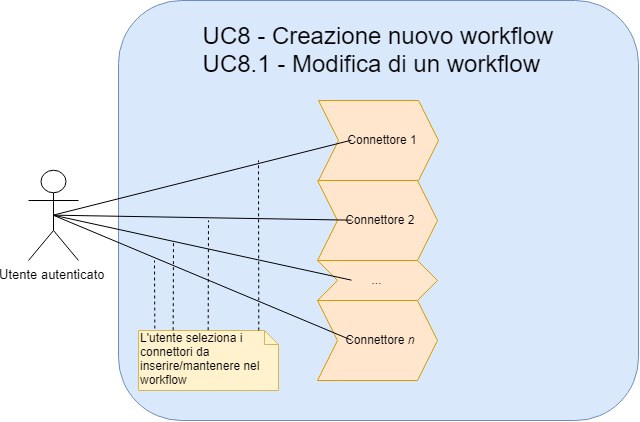
\includegraphics[width=13cm,keepaspectratio]{../includes/pics/Creazione_modifica_workflow.png}
%%%	\caption{\label{fig:mission}Creazione e modifica di un workflow}
%%%\end{figure}
%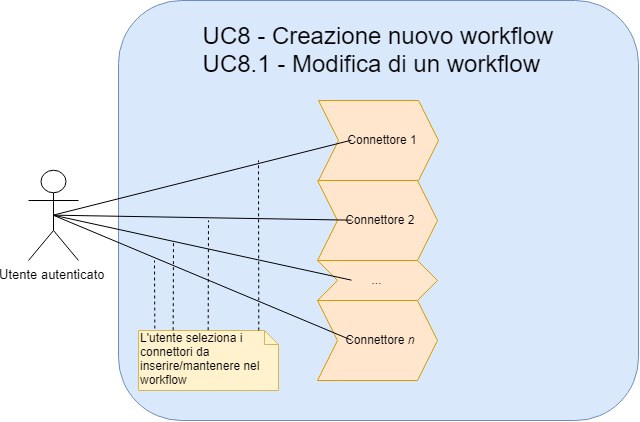
\includegraphics[width=1\textwidth]{../includes/pics/Creazione_modifica_workflow.png}

\subsubsection{UC7 - Creazione nuovo workflow}
\begin{itemize}
	\item  Attori primari: utente autenticato;
	\item  Scopo e descrizione: l'utente crea un nuovo workflow;
	\item  Scenario principale: l'utente preme il bottone per aggiungere un nuovo workflow e sceglie un nome identificativo per il workflow.
	\item  Pre-condizione: l'utente vuole creare un nuovo workflow;
	\item  Post-condizione: l'utente ha creato un nuovo workflow associato al proprio account.
\end{itemize}

\begin{figure}[H]
	\centering
	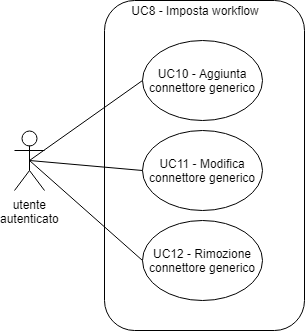
\includegraphics[width=15cm,keepaspectratio]{../includes/pics/imposta_workflow.png}
	\caption{\label{fig:mission}UC8 - Imposta workflow}
\end{figure}

\subsubsection{UC8 - Imposta workflow}
\begin{itemize}
	\item  Attori primari: utente autenticato;
	\item  Scopo e descrizione: l'utente imposta un workflow esistente;
	\item  Scenario principale:  
	\begin{enumerate}
		\item l'utente visualizza la lista di connettori proposti;
		 %%problema sottocasi cardin
		\item sceglie quali connettori aggiungere, modificare o eventualmente eliminare;
		\item imposta i connettori nuovi o modificati;
		\item può scegliere un nuovo ordine per i connettori;
		\item associa per la prima volta o modifica un comando vocale e\textbackslash o testuale associato per l'avvio del workflow;
		\item crea o modifica il nome del workflow.
	\end{enumerate}
	\item  Pre-condizione: l'utente vuole impostare un workflow;
	\item  Post-condizione: l'utente ha impostato un workflow associato al proprio account.
\end{itemize}
\subsubsection{UC9 - Rimozione workflow}
\begin{itemize}
	\item  Attori primari: utente autenticato;
	\item  Scopo e descrizione: l'utente elimina un workflow già creato;
	\item  Scenario principale: l'utente visualizza la lista di workflow associati al proprio account e tramite un comando elimina un determinato workflow liberando anche il nome associato a quest'ultimo;
	\item  Pre-condizione: esiste almeno un workflow, l'utente vuole rimuovere tale workflow;
	\item  Post-condizione: l'utente ha rimosso un workflow associato al proprio account.
\end{itemize}

\begin{figure}[H]
	\centering
	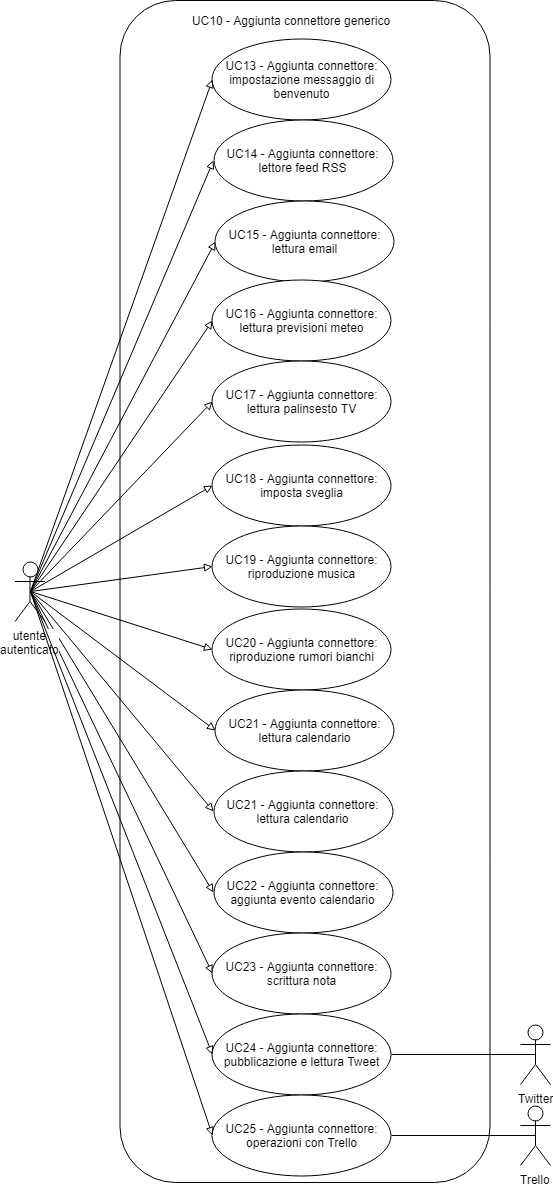
\includegraphics[width=10cm,keepaspectratio]{../includes/pics/aggiunta_connettore_generico.png}
	\caption{\label{fig:mission}UC10 - Aggiunta connettore generico}
\end{figure}

\subsubsection{UC10 - Aggiunta connettore generico}
\begin{itemize}
	\item  Attori primari: utente autenticato;
	\item  Scopo e descrizione: l'utente aggiunge un connettore ad un workflow;
	\item  Scenario principale: l'utente visualizza la lista di connettori proposti, dopo averne scelto uno imposta eventuali opzioni aggiuntive, il connettore viene quindi aggiunto al workflow;
	\item  Pre-condizione: l'utente vuole aggiungere un connettore al workflow;
	\item  Post-condizione: l'utente ha impostato il connettore e questo è stato aggiunto al workflow associato al proprio account.
\end{itemize}
\subsubsection{UC11 - Modifica connettore generico}
\begin{itemize}
	\item  Attori primari: utente autenticato;
	\item  Scopo e descrizione: l'utente modifica un connettore presente in un workflow;
	\item  Scenario principale: l'utente visualizza la lista di connettori del workflow, dopo averne scelto uno può modificare le opzioni aggiuntive dello stesso, il connettore modificato viene quindi aggiunto al workflow al posto del precedente;
	\item  Pre-condizione: esiste almeno un connettore nel workflow, l'utente vuole modificare tale connettore del workflow;
	\item  Post-condizione: l'utente ha impostato il connettore e questo è stato aggiunto al workflow sostituendo il vecchio connettore.
\end{itemize}
\subsubsection{UC12 - Rimozione connettore generico}
\begin{itemize}
	\item  Attori primari: utente autenticato;
	\item  Scopo e descrizione: l'utente modifica un workflow rimuovendo uno o più connettori;
	\item  Scenario principale: l'utente visualizza la lista di connettori del workflow, tramite un apposito comando elimina uno o più connettori presenti nel workflow ;
	\item  Pre-condizione: esiste almeno un connettore nel workflow, l'utente vuole eliminare tale connettore dal workflow;
	\item  Post-condizione: l'utente ha modificato il workflow eliminando il connettore scelto.
\end{itemize}
\subsubsection{UC13 - Aggiunta connettore: impostazione messaggio di benvenuto}
\begin{itemize}
	\item  Attori primari: utente autenticato;
	\item  Scopo e descrizione: permette di impostare un messaggio di benvenuto associato al workflow che si andrà a creare;
	\item  Voice flow dell'assistente vocale: l'assistente comunica il testo scelto dall'utente come messaggio di benvenuto;
	\item  Pre-condizione: l'utente è autenticato, il sistema è funzionante e raggiungibile, si sta creando un workflow;
	\item  Post-condizione: l'utente ha impostato un messaggio di benvenuto per il workflow corrente.
\end{itemize}
%\begin{figure}[H]
%	\centering
%	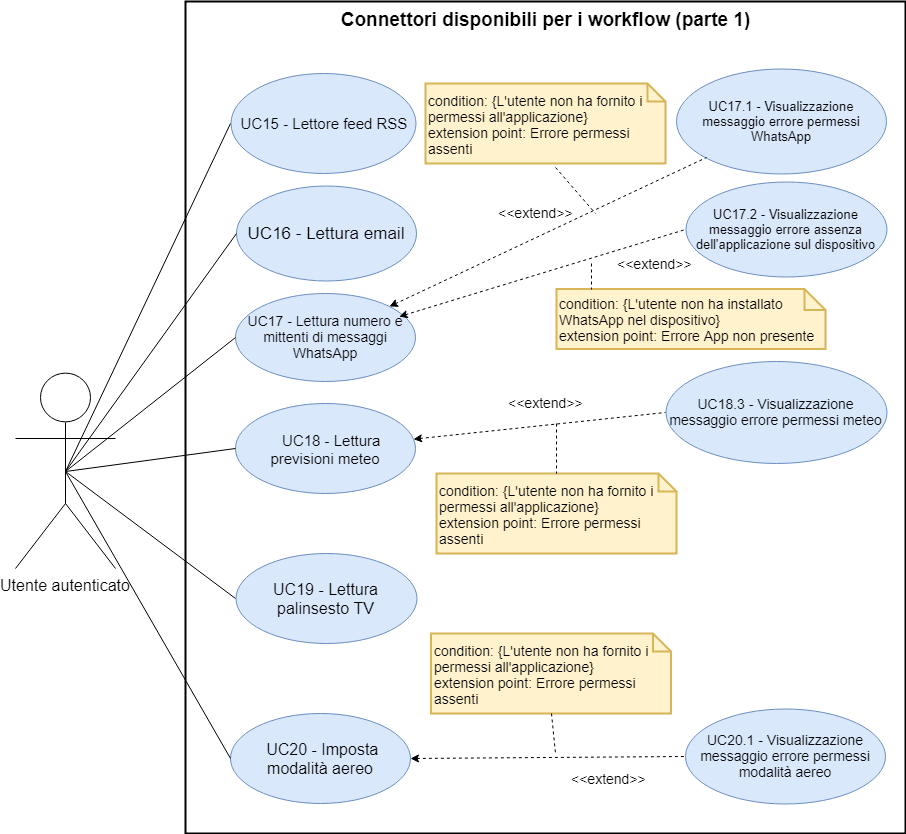
\includegraphics[width=15cm,keepaspectratio]{../includes/pics/wf1.png}
%	\caption{\label{fig:mission}connettori disponibili [UC13] - [UC25]}
%\end{figure}
%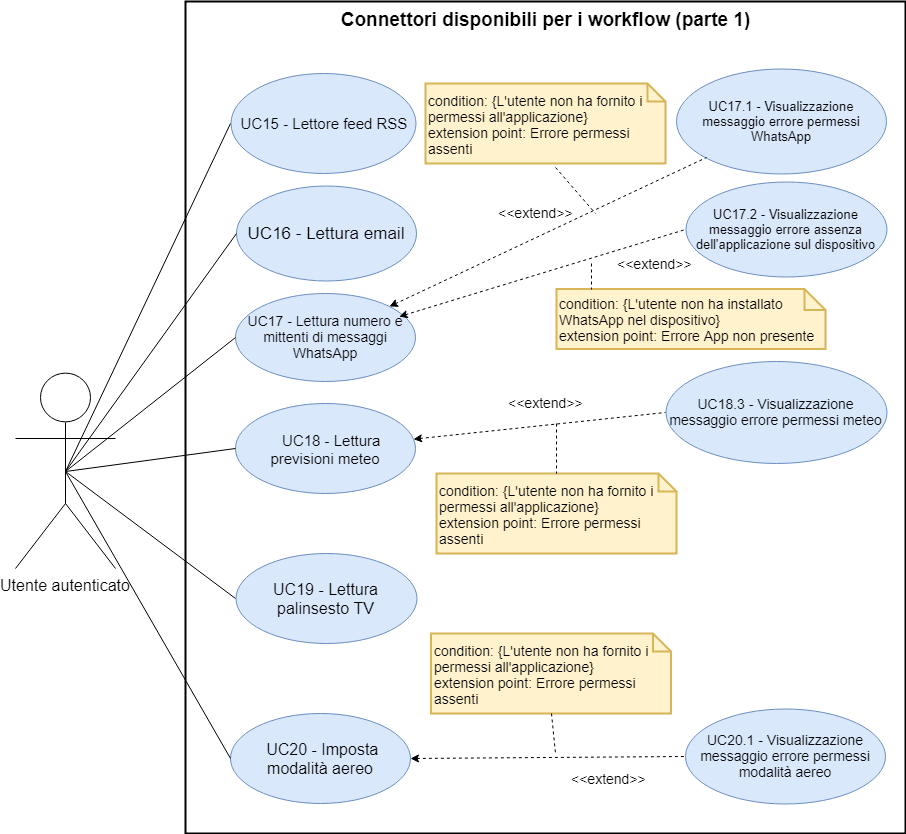
\includegraphics[width=1\textwidth]{../includes/pics/wf1.png}

\subsubsection{UC14 - Aggiunta connettore: lettore feed RSS}
\begin{itemize}
	\item  Attori primari: utente autenticato;
	\item  Scopo e descrizione: permette all'assistente vocale di leggere un feed RSS impostato dall'utente tramite digitazione di un URL, è inoltre possibile impostare un filtro per parole chiave [UC14.1];%%\addref{sec:UC9.4.1};%%\hyperref[sec:UC9.4.1]{UC9.4.1};
	\item  Voice flow dell'assistente vocale: l'assistente comunica il contenuto dell'ultimo feed RSS ricevuto;
	\item  Pre-condizione: l'utente è autenticato, il sistema è funzionante e raggiungibile, si sta creando/modificando un workflow;
	\item  Post-condizione: l'utente ha impostato un connettore che si occupa di leggere un feed RSS.
\end{itemize}
%\begin{itemize}
	%\item  Attori primari: utente autenticato;
	%\item  Scopo e descrizione: vengono presentate regole impostabili che fungono da criterio per filtrare feed RSS di un connettore per la lettura dei feed RSS;
	%\item  Voice flow dell'assistente vocale: l'assistente comunica il contenuto dell'ultimo feed RSS filtrato secondo i criteri impostati;
	%\item  Pre-condizione: il sistema è funzionante e raggiungibile, si sta creando/modificando un workflow, nel workflow corrente è presente un connettore per la lettura di feed RSS;
	%\item  Post-condizione: l'utente ha impostato dei criteri per filtrare un feed RSS.
%\end{itemize}
%\subsubsection{UC14.1 - Parole chiave filtro feed RSS}
%\begin{itemize}
%	\item  Attori primari: utente autenticato;
%	\item  Scopo e descrizione: viene presentato un campo in cui l'utente può digitare parole chiave separate da uno spazio, il sistema provvederà a cercare solo le notizie contententi/relative a queste;
%	\item  Pre-condizione: il sistema è funzionante e raggiungibile, si sta creando/modificando un workflow, nel workflow corrente è presente un connettore per la lettura di feed RSS;
%	\item  Post-condizione: l'utente ha impostato delle parole chiave per filtrare un feed RSS.
%\end{itemize}
%\subsubsection{UC15 - Aggiunta connettore: lettura email}
%\begin{itemize}
%	\item  Attori primari: utente autenticato;
%	\item  Scopo e descrizione: permette di associare un indirizzo di posta elettronica al connettore, verranno estratti mittenti e titoli delle email non aperte arrivate nelle ultime 24 ore;
%	\item  Voice flow dell'assistente vocale: l'assistente comunica titoli e mittenti delle email marcate come non lette arrivate nelle ultime 24 ore;
%	\item  Pre-condizione: l'utente è autenticato, il sistema è funzionante e raggiungibile, si sta creando/modificando un workflow;
%	\item  Post-condizione: l'utente ha impostato un connettore per ricevere feedback vocali riferiti a una casella di posta elettronica.
%\end{itemize}
%\subsubsection{UC15.1 - Associazione casella di posta elettronica}
%\begin{itemize}
%	\item  Attori primari: utente autenticato;
%	\item  Scopo e descrizione: viene mostrata all'utente una lista di servizi di posta elettronica, questo sceglie il proprio provider, viene quindi presentato un form con i campi indirizzo email e password, l'utente dovrà fornire queste credenziali.
%	\item  Scenario principale: l'utente sceglie il provider e fornisce le credenziali per accedere alla casella di posta elettronica;
%	\item  Estensioni:
%		   \begin{itemize}
%				\item  se l'utente non fornisce provider e/o credenziali di un account di posta elettronica valido riceve un messaggio di errore [UC15.1.1];
%		   \end{itemize}
%	\item  Pre-condizione: il sistema è funzionante e raggiungibile, si sta creando/modificando un workflow, si sta impostando un connettore: lettura email [UC15];
%	\item  Post-condizione: l'utente ha associato un account email al connettore: lettura email;
%\end{itemize}
%\subsubsection{UC15.1.1 - Visualizzazione messaggio errore di accesso account posta elettronica}
%\begin{itemize}
%	\item  Attori primari: utente autenticato;
%	\item  Scopo e descrizione: l'utente viene avvisato di non poter effettuare l'associazione all'account email;
%	\item  Scenario principale: l'utente visualizza l'errore relativo al mancato accesso all'account;
%	\item  Pre-condizione: l'utente vuole associare un account email fornendo dati errati;
%	\item  Post-condizione: l'utente è consapevole di dover fornire dati associati ad un account valido;
%\end{itemize}
%\subsubsection{UC16 - Aggiunta connettore: lettura numero e mittenti di messaggi WhatsApp}
%\begin{itemize}
%	\item  Attori primari: utente autenticato;
%	\item  Scopo e descrizione: connettore non impostabile, se trova installato sul dispositivo WhatsApp, estrae numero di messaggi non letti e relativi mittenti;
%	\item  Voice flow dell'assistente vocale: l'assistente comunica, in ordine, numero di messaggi non letti e relativo mittente, per ogni mittente associato a messaggi non letti;
%	\item  Estensioni:
%		   \begin{itemize}
%				\item se l'utente non fornisce all'applicazione i permessi necessari riceve un messaggio di errore [UC16.1];
%				\item se l'utente non possiede WhatsApp come applicazione installata nel dispositivo, riceve un messaggio di errore [UC16.2].
%		   \end{itemize}
%	\item  Pre-condizione: l'utente è autenticato,il sistema è funzionante e raggiungibile, si sta creando/modificando un workflow;
%	\item  Post-condizione: l'utente ha impostato un connettore per ricevere feedback vocali dei messaggi WhatsApp ricevuti.
%\end{itemize}
%\subsubsection{UC16.1 - Visualizzazione messaggio errore permessi WhatsApp}
%\begin{itemize}
%	\item  Attori primari: utente autenticato;
%	\item  Scopo e descrizione: l'utente viene avvisato di non poter aggiungere il connettore senza aver fornito i permessi necessari all'applicazione;
%	\item  Scenario principale: l'utente visualizza l'errore relativo alla mancanza di permessi;
%	\item  Pre-condizione: l'utente vuole aggiungere un connettore senza aver fornito i permessi;
%	\item  Post-condizione: l'utente è consapevole di dover fornire i permessi necessari per poter utilizzare il %connettore.
%\end{itemize}
%\subsubsection{UC16.2 - Visualizzazione messaggio errore assenza dell'applicazione WhatsApp sul dispositivo}
%\begin{itemize}
%	\item  Attori primari: utente autenticato;
%	\item  Scopo e descrizione: l'utente viene avvisato della mancanza dell'applicazione WhatsApp sul dispositivo;
%	\item  Scenario principale: l'utente visualizza l'errore relativo alla necessità di dover installare WhatsApp sul dispositivo per poter utilizzare il connettore;
%	\item  Pre-condizione: l'utente vuole aggiungere un connettore senza che WhatsApp sia installato sul dispositivo;
%	\item  Post-condizione: l'utente è consapevole di dover installare l'applicazione per poter disporre del connettore %per la lettura di messaggi WhatsApp [UC16].
%\end{itemize}
\subsubsection{UC15 - Aggiunta connettore: lettura previsioni meteo}
\begin{itemize}
	\item  Attori primari: utente autenticato;
	\item  Scopo e descrizione: permette di impostare una posizione tramite inserimento del nome di un comune o tramite geolocalizzazione del dispositivo Android. Di questa posizione verranno comunicate le condizioni meteorologiche;
	\item  Voice flow dell'assistente vocale: l'assistente comunica precipitazioni e temperature riferite alle 36 ore successive dell'area impostata dal connettore;
	\item  Estensioni: 
		   \begin{itemize}
				\item se l'utente non fornisce all'applicazione i permessi necessari riceve un messaggio di errore [UC15.3].
		   \end{itemize}
	\item  Pre-condizione: l'utente è autenticato, il sistema è funzionante e raggiungibile, si sta creando/modificando un workflow;
	\item  Post-condizione: l'utente ha impostato un connettore per ricevere informazioni meteorologiche.
\end{itemize}
\subsubsection{UC15.1 - Inserimento posizione manuale}
\begin{itemize}
	\item  Attori primari: utente autenticato;
	\item  Scopo e descrizione: viene presentato all'utente un campo in cui può digitare la sua posizione (città);
	\item  Pre-condizione: l'utente è autenticato, il sistema è funzionante e raggiungibile, si sta creando/modificando un workflow e si sta impostando un connettore: lettura previsioni meteo;
	\item  Post-condizione: l'utente ha fornito una posizione di cui vuole sapere le previsioni meteo.
\end{itemize}
\subsubsection{UC15.2 - Inserimento posizione tramite geolocalizzazione}
\begin{itemize}
	\item  Attori primari: utente autenticato;
	\item  Scopo e descrizione: viene presentato all'utente un bottone che alla pressione permette al sistema di salvare la posizione tramite geolocalizzazione;
	\item  Pre-condizione: l'utente è autenticato, il sistema è funzionante e raggiungibile, si sta creando/modificando un workflow e si sta impostando un connettore: lettura previsioni meteo;
	\item  Post-condizione: l'utente ha fornito una posizione di cui vuole sapere le previsioni meteo.
\end{itemize}
\subsubsection{UC15.3 - Visualizzazione messaggio errore permessi meteo}
\begin{itemize}
	\item  Attori primari: utente autenticato;
	\item  Scopo e descrizione: l'utente viene avvisato di non poter aggiungere il connettore senza aver fornito i permessi necessari all'applicazione;
	\item  Scenario principale: l'utente visualizza l'errore relativo alla mancanza di permessi;
	\item  Pre-condizione: l'utente vuole aggiungere un connettore meteo riferito alla posizione del dispositivo Android senza aver fornito i permessi;
	\item  Post-condizione: l'utente è consapevole di dover fornire i permessi necessari per poter utilizzare il connettore.
\end{itemize}
\subsubsection{UC16 - Aggiunta connettore: lettura palinsesto TV}
\begin{itemize}
	\item  Attori primari: utente autenticato;
	\item  Scopo e descrizione: permette di selezionare alcuni canali in chiaro di cui si vuole sapere la programmazione, va inoltre specificata la fascia oraria;
	\item  Voice flow dell'assistente vocale: l'assistente comunica, in ordine numerico, le trasmissioni dei canali scelti, che vanno in onda nella fascia oraria scelta;
	\item  Pre-condizione: l'utente è autenticato, il sistema è funzionante e raggiungibile, si sta creando/modificando un workflow;
	\item  Post-condizione: l'utente ha impostato un connettore per ricevere informazioni su una parte del palinsesto televisivo.
\end{itemize}
\subsubsection{UC16.1 impostazione canali per lettura palinsesto TV}
\begin{itemize}
	\item  Attori primari: utente autenticato;
	\item  Scopo e descrizione: viene presentata all'utente una lista di palinsesti (Rai, Mediaset, Premium, Sky, solo film), riceverà informazioni dall'assistente vocale solo dei canali scelti;
	\item  Pre-condizione: l'utente è autenticato, il sistema è funzionante e raggiungibile, si sta creando/modificando un workflow e si sta impostando un connettore: lettura palinsesto TV;
	\item  Post-condizione: l'utente ha impostato i palinsesti TV di cui vuole ricevere informazioni.
\end{itemize}
%\subsubsection{UC18 - Aggiunta connettore: imposta modalità aereo}
%\begin{itemize}
%	\item  Attori primari: utente autenticato;
%	\item  Scopo e descrizione: connettore non impostabile, permette di mettere in modalità aereo il dispositivo Android su cui si sta eseguendo il sistema;
%	\item  Voice flow dell'assistente vocale: l'assistente comunica che il dispositivo è entrato in modalità aereo;
%	\item  Estensioni: 
%		   \begin{itemize}
%				\item se l'utente non fornisce all'applicazione i permessi necessari riceve un messaggio di errore [UC18.1].
%		   \end{itemize}
%	\item  Pre-condizione: l'utente è autenticato, il sistema è funzionante e raggiungibile, si sta creando un workflow;
%	\item  Post-condizione: l'utente ha impostato un connettore che quando verrà eseguito porrà il dispositivo Android in modalità aereo.
%\end{itemize}
%\subsubsection{UC19.1 - Visualizzazione messaggio errore permessi modalità aereo}
%\begin{itemize}
%	\item  Attori primari: utente autenticato;
%	\item  Scopo e descrizione: l'utente viene avvisato di non poter aggiungere il connettore senza aver fornito i permessi necessari all'applicazione;
%	\item  Scenario principale: l'utente visualizza l'errore relativo alla mancanza di permessi;
%	\item  Pre-condizione: l'utente vuole aggiungere un connettore riferito all'attivazione della modalità aereo del dispositivo Android senza aver fornito i permessi;
%	\item  Post-condizione: l'utente è consapevole di dover fornire i permessi necessari per poter utilizzare il connettore.
%\end{itemize}

%\begin{figure}[H]
%	\centering
%	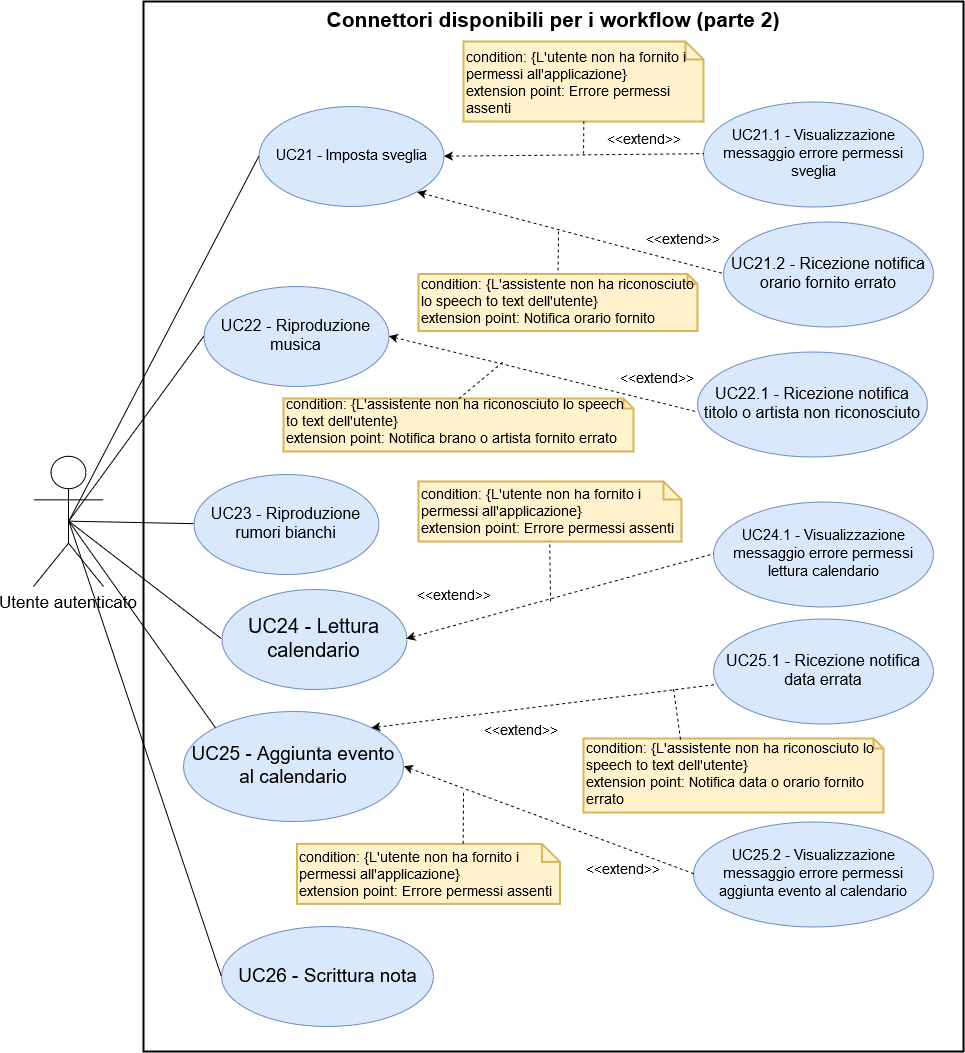
\includegraphics[width=15cm,keepaspectratio]{../includes/pics/wf2.png}
%	\caption{\label{fig:mission}connettori disponibili [UC21] - [UC26]}
%\end{figure}
%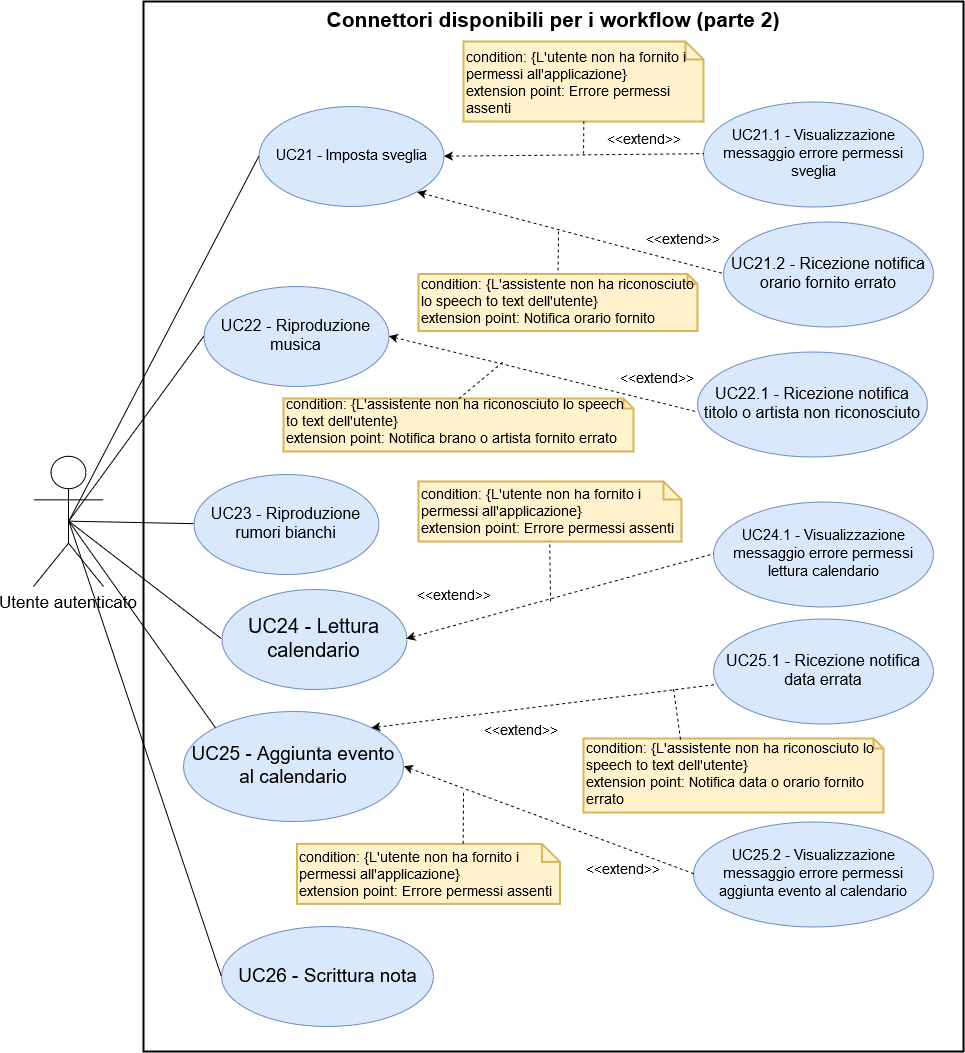
\includegraphics[width=1\textwidth]{../includes/pics/wf2.png}
%\clearpage
%\subsubsection{UC18 - Aggiunta connettore: imposta sveglia}
%\begin{itemize}
%	\item  Attori primari: utente autenticato;
%	\item  Scopo e descrizione: permette di impostare un orario per la sveglia che verrà attivata alla chiamata del workflow in cui questo connettore è contenuto;
%	\item  Voice flow dell'assistente vocale: l'assistente chiede se c'e l'intenzione di impostare una sveglia, se la risposta e' positiva continua chiedendo l'orario da impostare;
	%\item  Estensioni: 
%		   \begin{itemize}
%				\item se l'utente non fornisce all'applicazione i permessi necessari riceve un messaggio di errore [UC18.1];
%				\item se l'utente durante lo speech-to-text fornisce un orario errato riceve una notifica vocale [UC18.2].
%		   \end{itemize}
%	\item  Pre-condizione: l'utente è autenticato, il sistema è funzionante e raggiungibile, si sta creando/modificando un workflow;
%	\item  Post-condizione: l'utente ha impostato un connettore che quando verrà eseguito attiverà la sveglia sul dispositivo associato.
%\end{itemize}
%\subsubsection{UC18.1 - Visualizzazione messaggio errore permessi imposta sveglia}
%\begin{itemize}
%	\item  Attori primari: utente autenticato;
%	\item  Scopo e descrizione: l'utente viene avvisato di non poter aggiungere il connettore senza aver fornito i permessi necessari all'applicazione;
%	\item  Scenario principale: l'utente visualizza l'errore relativo alla mancanza di permessi;
%	\item  Pre-condizione: l'utente vuole aggiungere un connettore riferito all'impostazione di una sveglia del dispositivo Android senza aver fornito i permessi;
%	\item  Post-condizione: l'utente è consapevole di dover fornire i permessi necessari per poter utilizzare il connettore.
%\end{itemize}
%\subsubsection{UC18.2 - Ricezione notifica orario errato}
%\begin{itemize}
%	\item  Attori primari: utente autenticato;
%	\item  Scopo e descrizione: l'utente tramite speech-to-text ha fornito un orario errato;
%	\item  Scenario principale: l'utente viene notificato della scelta errata dell'orario;
%	\item  Voice flow dell'assistente vocale: l'assistente notifica che l'utente ha impostato un orario sbagliato, comunica quindi se l'utente vuole reimpostare la sveglia;
%	\item  Pre-condizione: l'utente ha scelto un orario errato;
%	\item  Post-condizione: l'utente è consapevole di dover ripetere l'iterazione per impostare l'orario della sveglia.
%\end{itemize}
%\subsubsection{UC19 - Aggiunta connettore: riproduzione musica}
%\begin{itemize}
%	\item  Attori primari: utente autenticato;
%	\item  Scopo e descrizione: permette di ascoltare un brano a scelta dell'utente;
%	\item  Voice flow dell'assistente vocale: l'assistente chiede all'utente il brano o l'artista che desidera ascoltare, dopo aver ricevuto una risposta comincia la riproduzione musicale;
%	\item  Estensioni:
%		   \begin{itemize}
%				\item se l'utente fornisce un titolo o un artista errato, riceve una notifica vocale [UC19.1].
%		   \end{itemize}
%	\item  Pre-condizione: l'utente è autenticato, il sistema è funzionante e raggiungibile, si sta creando/modificando un workflow;
%	\item  Post-condizione: l'utente ha impostato un connettore che quando verrà eseguito avvierà la riproduzione musicale dal dispositivo.
%\end{itemize}
%\subsubsection{UC19.1 - Ricezione notifica titolo o artista non riconosciuto}
%\begin{itemize}
%	\item  Attori primari: utente autenticato;
%	\item  Scopo e descrizione: l'utente viene avvisato che il titolo o l'artista richiesto non è stato riconosciuto dall'assistente;
%	\item  Scenario principale: l'utente riceve l'errore relativo all'errato riconoscimento da parte dell'assistente;
%	\item  Pre-condizione: l'utente vuole aggiungere un connettore al workflow che permetta di avviare una riproduzione musicale specificando il titolo o l'artista;
%	\item  Post-condizione: l'utente è consapevole di dover fornire il titolo o l'artista in un formato corretto per poter utilizzare il connettore.
%\end{itemize}
%\subsubsection{UC19 - Aggiunta connettore: riproduzione rumori bianchi}
%\begin{itemize}
%	\item  Attori primari: utente autenticato;
%	\item  Scopo e descrizione: permette di impostare una durata di tempo, durante la quale, a workflow chiamato, verrà riprodotta una playlist di rumori bianchi;%TODO in locale o da internet?
%	\item  Voice flow dell'assistente vocale: l'assistente riproduce la playlist di suoni scelti;
%	\item  Pre-condizione: l'utente è autenticato, il sistema è funzionante e raggiungibile, si sta creando/modificando un workflow;
%	\item  Post-condizione: l'utente ha impostato un connettore che quando verrà eseguito riprodurrà una playlist di rumori bianchi.
%\end{itemize}
%\subsubsection{UC21 - Aggiunta connettore: lettura calendario}
%\begin{itemize}
%	\item  Attori primari: utente autenticato;
%	\item  Scopo e descrizione: permette, all'esecuzione, di ricevere informazioni sui prossimi eventi del calendario;
%	\item  Voice flow dell'assistente vocale: l'assistente comunica gli eventi del giorno segnati sul calendario; al termine chiede all'utente se vuole sapere quali sono gli eventi dei giorni successivi;
%	\item  Estensioni: 
%		   \begin{itemize}
%				\item se l'utente non fornisce all'applicazione i permessi necessari riceve un messaggio di errore [UC21.1].
%		   \end{itemize}
%	\item  Pre-condizione: l'utente è autenticato,il sistema è funzionante e raggiungibile, si sta creando/modificando un workflow, è stato impostato il periodo di tempo di cui si vogliono ricevere notizie sugli eventi e si sono forniti i permessi necessari;
%	\item  Post-condizione: l'utente ha impostato un connettore che quando verrà eseguito permetterà il riepilogo degli eventi in programma.
%\end{itemize}
%\subsubsection{UC21.1 - Visualizzazione messaggio errore permessi lettura calendario}
%\begin{itemize}
%	\item  Attori primari: utente autenticato;
%	\item  Scopo e descrizione: l'utente viene avvisato di non poter aggiungere il connettore senza aver fornito i permessi necessari all'applicazione.
%	\item  Scenario principale: l'utente visualizza l'errore relativo alla mancanza di permessi.
%	\item  Pre-condizione: l'utente vuole aggiungere un connettore riferito alla lettura del calendario del dispositivo Android senza aver fornito i permessi.
%	\item  Post-condizione: l'utente è consapevole di dover fornire i permessi necessari per poter utilizzare il connettore.
%\end{itemize}
%\subsubsection{UC22 - Aggiunta connettore: aggiunta evento calendario}
%\begin{itemize}
%	\item  Attori primari: utente autenticato;
%	\item  Scopo e descrizione: permette, all'esecuzione, di aggiungere tramite speech-to-text un evento al calendario;
%	\item  Voice flow dell'assistente vocale: l'assistente domanda se esiste l'intenzione di aggiungere un evento da parte dell'utente, a risposta positiva chiede di proseguire con la data ed eventuali informazioni dell'evento;
%	\item  Estensioni: 
%		   \begin{itemize}
%			    \item se l'utente durante lo speech-to-text imposta una data errata, riceve una notifica vocale [UC22.1];
%				\item se l'utente non fornisce all'applicazione i permessi necessari riceve un messaggio di errore [UC22.2].
%		   \end{itemize}
%	\item  Pre-condizione: l'utente è autenticato,il sistema è funzionante e raggiungibile, si sta creando un workflow e si sono forniti i permessi necessari;
%	\item  Post-condizione: l'utente ha impostato un connettore che quando verrà eseguito permetterà l'aggiunta di un evento al calendario Google.
%\end{itemize}
%\subsubsection{UC22.1 - Ricezione notifica data errata}
%\begin{itemize}
%	\item  Attori primari: utente autenticato;
%	\item  Scopo e descrizione: l'utente ha impostato una data sbagliata, può quindi decidere se modificare la data o eliminare l'aggiunta dell'evento;
%	\item  Scenario principale: l'utente viene notificato dell'errata scelta della data;
%	\item  Voice flow dell'assistente vocale: l'assistente notifica che l'utente ha impostato una data sbagliata durante la fase di speech-to-text, continua quindi chiedendo se desidera modificare la data o eliminare l'aggiunta dell'evento al calendario;
%	\item  Pre-condizione: l'utente ha impostato una data sbagliata per un nuovo evento del calendario;
%	\item  Post-condizione: l'utente è consapevole di non poter scegliere date errate e che può modificare la data o eliminare l'evento.
%\end{itemize}
%\subsubsection{UC22.2 - Visualizzazione messaggio errore permessi aggiunta evento calendario}
%\begin{itemize}
%	\item  Attori primari: utente autenticato;
%	\item  Scopo e descrizione: l'utente viene avvisato di non poter aggiungere il connettore senza aver fornito i permessi necessari all'applicazione;
%	\item  Scenario principale: l'utente visualizza l'errore relativo alla mancanza di permessi;
%	\item  Pre-condizione: l'utente vuole aggiungere un connettore riferito all'aggiunta di un evento al calendario del dispositivo Android senza aver fornito i permessi;
%	\item  Post-condizione: l'utente è consapevole di dover fornire i permessi necessari per poter utilizzare il connettore.
%\end{itemize}
%\subsubsection{UC23 - Aggiunta connettore: scrittura nota}
%\begin{itemize}
%	\item  Attori primari: utente autenticato;
%	\item  Scopo e descrizione: permette, all'esecuzione, di aggiungere una nota al telefono tramite speech-to-text, non vi è una limitazione alla lunghezza delle note;
%	\item  Voice flow dell'assistente vocale: l'assistente domanda se esiste l'intenzione di aggiungere una nuova nota da parte dell'utente, a risposta positiva chiede di proseguire con il corpo della nota;
%	\item  Pre-condizione: l'utente è autenticato,il sistema è funzionante e raggiungibile, si sta creando/modificando un workflow e sono stati forniti i permessi necessari;
%	\item  Post-condizione: l'utente ha impostato un connettore che quando verrà eseguito permetterà l'aggiunta di una nota.
%\end{itemize}

\begin{figure}[H]
	\centering
	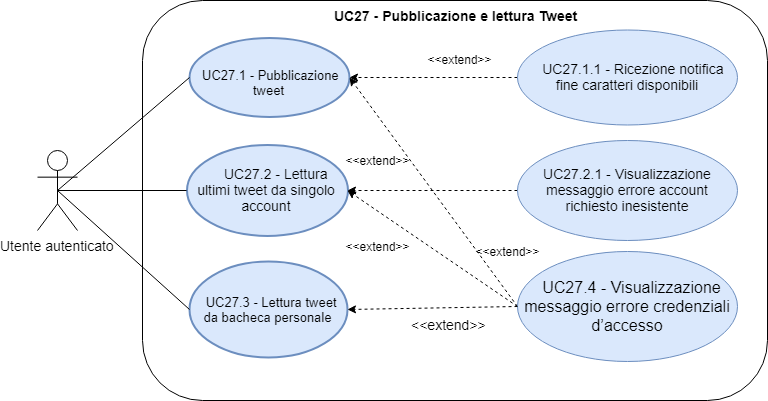
\includegraphics[width=14cm,keepaspectratio]{../includes/pics/connettore_twitter.png}
	\caption{\label{fig:mission}connettore Twitter}
\end{figure}
%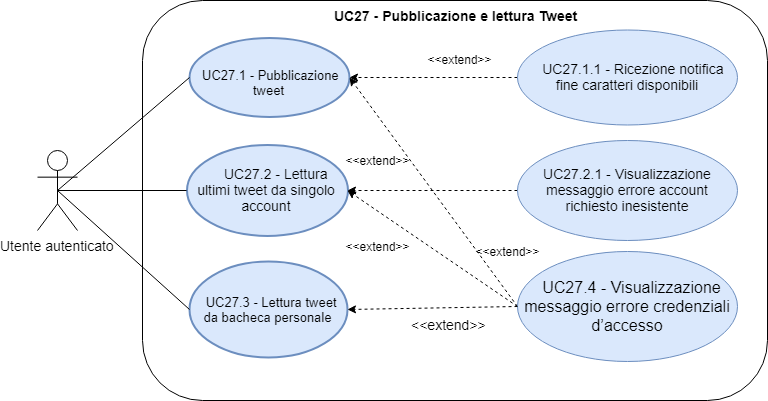
\includegraphics[width=1\textwidth]{../includes/pics/connettore_twitter.png}

\subsubsection{UC17 - Aggiunta connettore: pubblicazione e lettura Tweet}
\begin{itemize}
	\item  Attori primari: utente autenticato;
    \item  Attori secondari: Twitter;
	\item  Scopo e descrizione: l'utente all'esecuzione può scegliere come interagire con Twitter, in particolare:
		   \begin{itemize}
				\item pubblicare un tweet [UC17.1];
				\item leggere gli ultimi tweet pubblicati da un singolo account [UC17.2];
				\item leggere gli ultimi tweet presenti nella bacheca personale [UC17.3].
		   \end{itemize}
	\item  Voice flow dell'assistente vocale: l'assistente chiede all'utente in che modo vuole interagire con Twitter durante il workflow;
	\item  Estensioni: 
		   \begin{itemize}
				\item se l'utente non fornisce all'applicazione le credenziali d'accesso necessarie riceve un messaggio di errore [UC17.4];
		   \end{itemize}
	\item  Pre-condizione: l'utente è autenticato, il sistema è funzionante e raggiungibile, si sta creando un workflow, si è associato un account Twitter e si sono forniti i permessi necessari;
	\item  Post-condizione: l'utente ha impostato un connettore che quando verrà eseguito permetterà di interagire con Twitter durante il workflow.
\end{itemize}
\subsubsection{UC17.1 - Pubblicazione tweet}
\begin{itemize}
	\item  Attori primari: utente autenticato;
	\item  Scopo e descrizione: permette, all'esecuzione, di pubblicare un tweet tramite speech-to-text, testi più lunghi di 280 caratteri verranno troncati;
	\item  Voice flow dell'assistente vocale: l'assistente chiede di ascoltare il corpo del tweet;
	\item  Estensioni: 
		   \begin{itemize}
				\item se l'utente durante lo speech-to-text supera i 280 caratteri, riceve una notifica vocale [UC17.1.1].
		   \end{itemize}
	\item  Pre-condizione: l'utente è autenticato,il sistema è funzionante e raggiungibile, si sta creando un workflow, si è associato un account Twitter e si sono forniti i permessi necessari;
	\item  Post-condizione: l'utente ha impostato un connettore che quando verrà eseguito permetterà la pubblicazione di un tweet.
\end{itemize}
\subsubsection{UC17.1.1 - Ricezione notifica fine caratteri disponibili}
\begin{itemize}
	\item  Attori primari: utente autenticato;
	\item  Scopo e descrizione: l'utente ha utilizzato tutti i 280 caratteri disponibili, può quindi decidere se inviare il messaggio, modificarlo o eliminarlo;
	\item  Scenario principale: l'utente viene notificato del raggiungimento del tetto limite di caratteri disponibili per il tweet;
	\item  Voice flow dell'assistente vocale: l'assistente notifica che l'utente ha terminato la fase di speech-to-text, continua quindi chiedendo se desidera: inviare il tweet, modificarlo facendo ricominciare lo speech-to-text oppure eliminare completamente il corpo del tweet;
	\item  Pre-condizione: l'utente ha raggiunto il tetto massimo di caratteri impostati per il corpo di un tweet;
	\item  Post-condizione: l'utente è consapevole di non poter più aggiungere altro testo al tweet e che può inviare, modificare o eliminare il messaggio.
\end{itemize}
\subsubsection{UC17.2 - Lettura ultimi tweet da singolo account}
\begin{itemize}
	\item  Attori primari: utente autenticato;
	\item  Scopo e descrizione: permette, all'esecuzione, di leggere gli ultimi tweet pubblicati da parte di un account. L'utente può durante l'ascolto scegliere di rispondere ad un tweet pubblicando una risposta [UC17.1];
	\item  Voice flow dell'assistente vocale: l'assistente comunica che andrà a leggere i tweet dell'utente impostato, quindi ne comincia la lettura tramite text to speech. Nel caso l'utente voglia scrivere un tweet di risposta l'assistente chiede di proseguire dettando il corpo del tweet [UC17.1];
	\item  Estensioni: 
		   \begin{itemize}
				\item se l'utente fornisce all'applicazione il nome di un account errato, riceve un messaggio di errore [UC17.2.1];
		   \end{itemize}
	\item  Pre-condizione: l'utente è autenticato,il sistema è funzionante e raggiungibile, si sta creando un workflow, si è associato un account Twitter, è stato impostato l'account e si sono forniti i permessi necessari;
	\item  Post-condizione: l'utente ha impostato un connettore che quando verrà eseguito permetterà di ascoltare gli ultimi tweet di un certo utente prestabilito.
\end{itemize}
\subsubsection{UC17.2.1 - Visualizzazione messaggio errore account Twitter richiesto inesistente}
\begin{itemize}
	\item  Attori primari: utente non autenticato;
	\item  Scopo e descrizione: l'utente viene avvisato che l'account inserito, di cui vuole ricevere i tweet pubblicati, non esiste;
	\item  Scenario principale: l'utente visualizza l'errore relativo all'errato inserimento del nome dell'account;
	\item  Pre-condizione: l'utente imposta il connettore inserendo il nome errato di un account;
	\item  Post-condizione: l'utente è consapevole di dover fornire il nome di un account Twitter esistente.
\end{itemize}
\subsubsection{UC17.3 - Lettura tweet bacheca personale}
\begin{itemize}
	\item  Attori primari: utente autenticato;
	\item  Scopo e descrizione: permette, all'esecuzione, di leggere gli ultimi tweet presenti nella bacheca personale. L'utente può durante l'ascolto scegliere di rispondere ad un tweet pubblicando una risposta [UC17.1];
	\item  Voice flow dell'assistente vocale: l'assistente comunica che andrà a leggere i tweet della bacheca personale dell'utente, ne comincia quindi la lettura tramite text to speech. Nel caso l'utente voglia scrivere un tweet di risposta l'assistente chiede di proseguire dettando il corpo del tweet [UC17.1];
	\item  Pre-condizione: l'utente è autenticato, il sistema è funzionante e raggiungibile, si sta creando/modificando un workflow;
	\item  Post-condizione: l'utente ha impostato un connettore che quando verrà eseguito permetterà di ascoltare gli ultimi tweet della bacheca personale dell'utente.
\end{itemize}
%\subsubsection{UC26.4 - Visualizzazione messaggio errore credenziali d'accesso}
%\begin{itemize}
%	\item  Attori primari: utente autenticato;
%	\item  Scopo e descrizione: l'utente viene avvisato di non poter aggiungere il connettore senza aver fornito le credenziali corrette per l'accesso all'account Twitter;
%	\item  Scenario principale: l'utente visualizza l'errore relativo alla mancanza di credenziali d'accesso;
%	\item  Pre-condizione: l'utente vuole aggiungere un connettore riferito all'invio di tweet senza aver fornito le credenziali dell'account;
%	\item  Post-condizione: l'utente è consapevole di dover fornire le credenziali corrette per poter utilizzare il connettore.
%\end{itemize}

\begin{figure}[H]
	\centering
	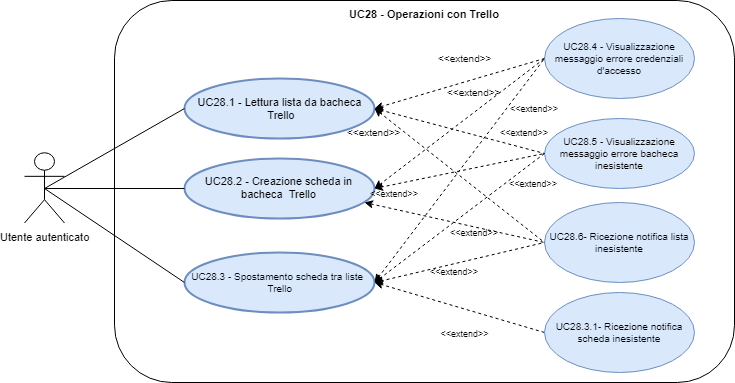
\includegraphics[width=14cm,keepaspectratio]{../includes/pics/trello.png}
	\caption{\label{fig:mission}connettore Trello}
\end{figure}
%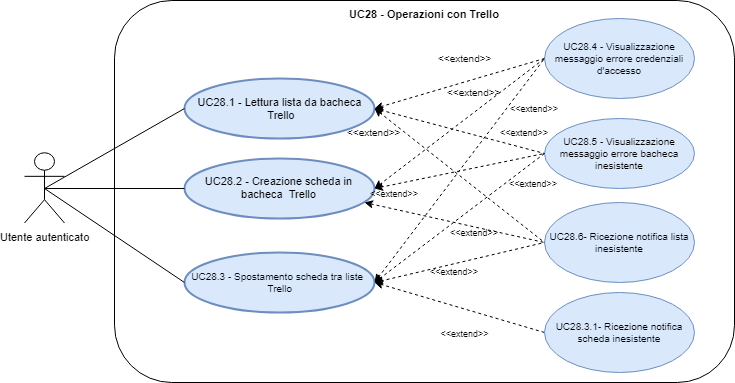
\includegraphics[width=1\textwidth]{../includes/pics/trello.png}

\subsubsection{UC18 - Aggiunta connettore: operazioni con Trello}
\begin{itemize}
	\item  Attori primari: utente autenticato;
     \item  Attori secondari: Trello;
	\item  Scopo e descrizione: l'utente all'esecuzione può scegliere come interagire con Trello, in particolare:
		   \begin{itemize}
				\item leggere le schede assegnate all'utente che sono presenti in una lista di una bacheca [UC18.1];
				\item creare una nuova scheda da aggiungere alla bacheca [UC18.2];
				\item spostare una scheda da una lista in un'altra lista della stessa bacheca [UC18.3].
		   \end{itemize}
	\item  Voice flow dell'assistente vocale: l'assistente chiede all'utente in che modo vuole interagire con Trello durante il workflow;
	\item  Estensioni: 
		   \begin{itemize}
				\item se l'utente non fornisce all'applicazione le credenziali d'accesso necessarie riceve un messaggio di errore [UC18.4];
				\item se l'utente fornisce all'applicazione il nome di una bacheca errata, riceve un messaggio di errore [UC18.5];
				\item se l'utente durante lo speech-to-text fornisce il nome di una lista non presente nella bacheca, riceve una notifica vocale [UC18.6];
		   \end{itemize}
	\item  Pre-condizione: l'utente è autenticato,il sistema è funzionante e raggiungibile, si sta creando/modificando un workflow, si è associato un account Trello e si sono forniti i permessi necessari;
	\item  Post-condizione: l'utente ha impostato un connettore che quando verrà eseguito permetterà di interagire con Trello durante il workflow.
\end{itemize}
\subsubsection{UC18.1 - Lettura lista da bacheca Trello}
\begin{itemize}
	\item  Attori primari: utente autenticato;
	\item  Scopo e descrizione: permette, all'esecuzione, di leggere le prime tre schede assegnate all'utente di una lista facente parte di una bacheca a scelta dell'utente;
	\item  Voice flow dell'assistente vocale: l'assistente domanda all'utente di quale lista desidera ricevere informazioni, dopo aver ricevuto risposta comincia la lettura tramite text-to-specch;
	\item  Pre-condizione: l'utente è autenticato, il sistema è funzionante e raggiungibile, si sta creando un workflow, si è associato un account Trello e si sono forniti i permessi necessari;
	\item  Post-condizione: l'utente ha impostato un connettore che quando verrà eseguito permetterà di ascoltare il contenuto delle schede di una lista facente parte di una bacheca prestabilita.
\end{itemize}
\subsubsection{UC18.2 - Creazione scheda in bacheca Trello}
\begin{itemize}
	\item  Attori primari: utente autenticato;
	\item  Scopo e descrizione: permette, all'esecuzione, di aggiungere una scheda ad una bacheca scelta precedentemente dall'utente;
	\item  Voice flow dell'assistente vocale: l' assistente vocale domanda il nome della lista in cui l'utente vuole aggiungere la scheda, l'utente quindi comunica il corpo della scheda tramite speech-to-text;
	\item  Pre-condizione: l'utente è autenticato, il sistema è funzionante e raggiungibile, si sta creando un workflow, si è associato un account Trello e si sono forniti i permessi necessari;
	\item  Post-condizione: l'utente ha impostato un connettore che quando verrà eseguito permetterà di aggiungere una nuova scheda ad una lista facente parte di una bacheca predefinita.
\end{itemize}
\subsubsection{UC18.3 - Spostamento scheda tra liste Trello}
\begin{itemize}
	\item  Attori primari: utente autenticato;
	\item  Scopo e descrizione: permette, all'esecuzione, di spostare una scheda in un'altra lista facente parte di una bacheca scelta precedentemente dall'utente;
	\item  Voice flow dell'assistente vocale: l'assistente vocale chiede il nome della lista da cui l'utente vuole spostare la scheda, il nome della scheda e il nome della lista su cui dovrà essere inserita la scheda;
	\item  Estensioni: 
		   \begin{itemize}
				\item se l'utente durante lo speech-to-text fornisce il nome di una scheda non presente nella bacheca, riceve una notifica vocale [UC18.3.1].
		   \end{itemize}
	\item  Pre-condizione: l'utente è autenticato, il sistema è funzionante e raggiungibile, si sta creando/modificando un workflow, si è associato un account Trello e si sono forniti i permessi necessari;
	\item  Post-condizione: l'utente ha impostato un connettore che quando verrà eseguito permetterà di spostare una scheda tra liste facenti parte di una bacheca prestabilita.
\end{itemize}
\subsubsection{UC18.3.1 - Ricezione notifica scheda inesistente}
\begin{itemize}
	\item  Attori primari: utente autenticato;
	\item  Scopo e descrizione: l'utente durante lo speech-to-text ha scelto una scheda che non è presente nella lista della bacheca impostata nel connettore, deve quindi scegliere di nuovo una scheda su cui eseguire i comandi;
	\item  Scenario principale: l'utente viene notificato dell'assenza della scheda richiesta;
	\item  Voice flow dell'assistente vocale: l'assistente notifica che l'utente durante la fase di speech-to-text ha fatto richiesta di una scheda inesistente, continua quindi chiedendo se desidera cambiare la scelta della scheda;
	\item  Pre-condizione: l'utente ha richiesto una scheda non presente nella lista della bacheca impostata nel connettore;
	\item  Post-condizione: l'utente è consapevole di aver richiesto una scheda inesistente e che può modificare la sua richiesta.
\end{itemize}
%\subsubsection{UC27.4 - Visualizzazione messaggio errore credenziali d'accesso}
%\begin{itemize}
%	\item  Attori primari: utente autenticato;
%	\item  Scopo e descrizione: l'utente viene avvisato di non poter aggiungere il connettore senza aver fornito le credenziali corrette per l'accesso all'account Trello;
%	\item  Scenario principale: l'utente visualizza l'errore relativo alla mancanza di credenziali d'accesso;
%	\item  Pre-condizione: l'utente vuole aggiungere un connettore riferito all'interazione con Trello senza aver fornito le credenziali dell'account;
%	\item  Post-condizione: l'utente è consapevole di dover fornire le credenziali corrette per poter utilizzare il connettore.
%\end{itemize}
\subsubsection{UC18.5 - Visualizzazione messaggio errore bacheca inesistente}
\begin{itemize}
	\item  Attori primari: utente autenticato;
	\item  Scopo e descrizione: l'utente viene avvisato che la bacheca inserita non risulta presente nell'account collegato;
	\item  Scenario principale: l'utente visualizza l'errore relativo all'errato inserimento del nome della bacheca;
	\item  Pre-condizione: l'utente imposta il connettore inserendo il nome errato di una bacheca;
	\item  Post-condizione: l'utente è consapevole di dover fornire il nome di una bacheca presente tra quelle dell'account collegato.
\end{itemize}
\subsubsection{UC18.6 - Ricezione notifica lista inesistente}
\begin{itemize}
	\item  Attori primari: utente autenticato;
	\item  Scopo e descrizione: l'utente durante lo speech-to-text ha scelto una lista che non è presente nella bacheca impostata nel connettore, deve quindi scegliere di nuovo una lista da cui ricevere informazioni;
	\item  Scenario principale: l'utente viene notificato dell'assenza della lista richiesta;
	\item  Voice flow dell'assistente vocale: l'assistente notifica che l'utente durante la fase di speech-to-text ha fatto richiesta di una lista inesistente, continua quindi chiedendo se desidera cambiare la scelta della lista;
	\item  Pre-condizione: l'utente ha richiesto una lista non presente nella bacheca impostata nel connettore;
	\item  Post-condizione: l'utente è consapevole di aver richiesto una lista inesistente e che può modificare la sua richiesta.
\end{itemize}
\subsubsection{UC19 - Attivazione vocale workflow}
\begin{itemize}
	\item Attori primari: utente autenticato;
	\item Scopo e descrizione: l'utente vuole avviare un workflow;
	\item Voice flow dell'assistente vocale: l'utente richiede tramite comando vocale all'assistente Amazon Alexa di avviare un workflow;
	\item Estensioni:
		se l'utente durante lo speech-to-text fornisce il nome di un workflow non presente nell'area personale dell'applicazione, riceve una notifica vocale [UC19.1].
	\item Pre-condizione: l'utente è autenticato, il sistema è funzionante e raggiungibile ed è stata avviata la skill relativa all'applicazione;
	\item Post-condizione: il workflow richiesto dall'utente è stato avviato: viene eseguito il primo connettore.
\end{itemize}
\subsubsection{UC19.1 - Ricezione notifica vocale workflow inesistente}
\begin{itemize}
	\item Attori primari: utente autenticato;
	\item Scopo e descrizione: l'utente durante lo speech-to-text ha scelto un workflow non presente nell'area personale dell'applicazione;
	\item Voice flow dell'assistente vocale: l'assistente notifica che l'utente durante la fase di speech-to-text ha richiesto l'avvio di un workflow inesistente;
	\item Pre-condizione: l'utente è autenticato ed ha richiesto l'avvio di un workflow inesistente;
	\item Post-condizione: l'utente è a conoscenza di aver richiesto un workflow non esistente.
\end{itemize}
\subsubsection{UC20 - Richiesta lista personale workflow}
\begin{itemize}
	\item Attori primari: utente autenticato;
	\item Scopo e descrizione: l'utente vuole conoscere la sua lista personale di workflow;
	\item Voice flow dell'assistente vocale: l'utente richiede tramite comando vocale all'assistente Amazon Alexa di elencare i suoi workflow personali; l'assistente risponde leggendo la lista;
	\item Pre-condizione: l'utente è autenticato, il sistema è funzionante e raggiungibile ed è stata avviata la skill relativa all'applicazione;
	\item Post-condizione: l'utente conosce la lista di workflow personali.
\end{itemize}
\subsubsection{UC21 - Richiesta aiuto}
\begin{itemize}
	\item Attori primari: utente autenticato;
	\item Scopo e descrizione: l'utente vuole ricevere un aiuto per utilizzare le funzionalità della skill;
	\item Voice flow dell'assistente vocale: l'utente richiede un aiuto tramite comando vocale all'assistente Amazon Alexa; l'assistente elenca le azioni che l'utente può effettuare;
	\item Pre-condizione: l'utente è autenticato, il sistema è funzionante e raggiungibile ed è stata avviata la skill relativa all'applicazione;
	\item Post-condizione: l'utente conosce la lista di funzionalità della skill.
\end{itemize}
\subsubsection{UC22 - Richiesta di termine della skill}
\begin{itemize}
	\item Attori primari: utente autenticato;
	\item Scopo e descrizione: l'utente vuole terminare la skill;
	\item Voice flow dell'assistente vocale: l'utente richiede ad Amazon Alexa l'interruzione della skill corrente;
	\item Pre-condizione: l'utente è autenticato, il sistema è funzionante e raggiungibile ed è stata avviata la skill relativa all'applicazione;
	\item Post-condizione: la skill viene interrotta.
\end{itemize}
\subsubsection{UC23 - Richiesta di termine del connettore corrente}
\begin{itemize}
	\item Attori primari: utente autenticato;
	\item Scopo e descrizione: l'utente vuole terminare il connettore attualmente in esecuzione;
	\item Voice flow dell'assistente vocale: l'utente richiede ad Amazon Alexa l'interruzione del connettore corrente;
	\item Pre-condizione: l'utente è autenticato, il sistema è funzionante e raggiungibile ed è stata avviata la skill relativa all'applicazione;
	\item Post-condizione: il connettore corrente viene interrotto e il workflow procede con il connettore seguente se presente.
\end{itemize}
\subsubsection{UC24 - Fallimento skill}
\begin{itemize}
	\item  Attori primari: utente autenticato;
	\item  Scopo e descrizione: l'utente viene notificato che Amazon Alexa non è riuscita a eseguire un connettore;
	\item  Pre-condizione: l'utente ha avviato un workflow e uno o più connettori sono falliti;
	\item  Post-condizione: l'utente è notificato del fatto che Amazon Alexa non è riuscita a portare a termine uno o più connettori del workflow avviato.
\end{itemize}